\section{Traffic, stairs and fleet}
\label{sec:traffic}

\begin{figure*}[t]
\centering
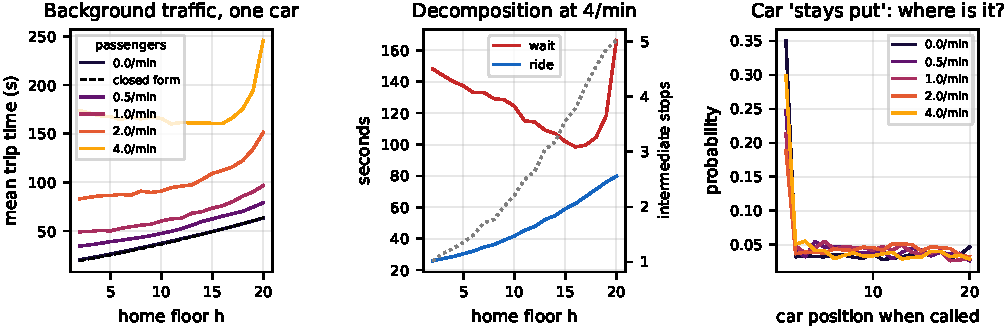
\includegraphics[width=\textwidth]{figures/traffic.pdf}
\caption{One car, lobby parking, $\alpha = \TraAlpha$, \TraN\ floors. Left:
mean trip time versus home floor for background rates from 0 to 4 passengers
per minute; the closed form (dashed) matches the simulator at zero traffic.
Middle: decomposition at 4/min --- the wait falls with height while the ride
and the number of intermediate stops rise. Right: where the car is when the
resident calls under the stay-put policy: the lobby dominates at every load.}
\label{fig:traffic}
\end{figure*}

\paragraph{Validation.} At zero traffic the simulator reproduces the closed
form to \TraValidErr\% mean relative error over all floors
(Figure~\ref{fig:traffic}, left), with the residual coming from the car
occasionally being caught mid-return to its parking floor.

\paragraph{Traffic flattens, then inverts.} Adding background passengers
raises every floor's time and compresses the curve: the regret of the middle
floor falls from \TraRegMidZero\% at zero traffic to \TraRegMidOne\% at
1/min and \TraRegMidTwo\% at 2/min, while the optimum stays at floor
\TraHTwo. At 4 passengers per minute a single car serving 20 floors is
saturated (best mean \TraBestFour\,s, of which most is waiting), and the
optimum jumps to floor \TraHFour\ with a middle-floor regret of only
\TraRegMidFour\%. The middle panel shows why. Under load the car sweeps the
building like a bus; a resident on a low floor who wants to go down is the
\emph{last} stop of the down sweep, so their wait (\TraHiWaitLow\,s on floor
2) exceeds that of a resident on floor \TraHiWaitMinFloor\
(\TraHiWaitMin\,s), and only the very top floor, served at the reversal, waits
longer still (\TraHiWaitTop\,s). Against that, the ride grows with height
(\TraHiRideLow\,s to \TraHiRideTop\,s) and collects up to \TraHiStopsTop\
intermediate stops. The two slopes nearly cancel over the middle of the
building, which is what ``it does not matter'' looks like in a saturated
system --- and the p90-optimal floor (\TraHpFour) remains low, because the
tail is made of the sweeps you miss.

\paragraph{Where the car actually is.} The right panel measures the stay-put
policy under traffic: the car is at the lobby \TraLastLobbyMassHalf\% of the
time at 0.5/min and \TraLastLobbyMass\% at 4/min, with the rest spread
almost uniformly. The stay-put policy is, in practice, a mixture of lobby
parking and the random-position limit --- which is why its optimum behaves
like the lobby-parking one at low load and drifts up (floor \TraLastHFour\ at
4/min) at high load.

\begin{figure}[t]
\centering
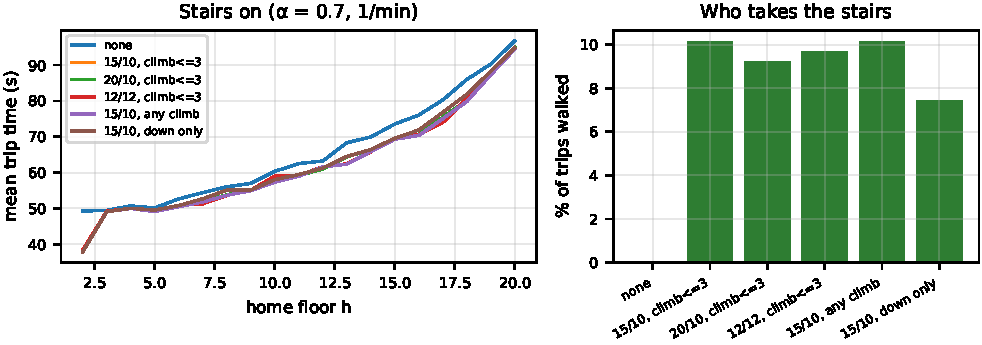
\includegraphics[width=\columnwidth]{figures/stairs.pdf}
\caption{Stairs at $\alpha = 0.7$, 1 passenger/min, one car. Left: mean trip
time by home floor for each stairs variant; right: fraction of trips walked.}
\label{fig:stairs}
\end{figure}

\paragraph{Stairs.} With the stairs available (15\,s up, 10\,s down, at most
three floors climbed) the best floor's mean time drops from \StaBestNone\ to
\StaBestOn\,s and \StaWalked\% of trips are walked, almost all of them the
one- and two-floor hops of a low-floor resident (Figure~\ref{fig:stairs}).
The optimum stays at floor \StaH\ at this lobby fraction, and the middle
floor's regret \emph{rises} from \StaRegMidNone\% to \StaRegMidOn\%, because
the stairs help the low floors most. The asymmetry we expected to matter does
not: a symmetric 12/12\,s stairs walks \StaWalkedSym\% of trips and a
descend-only resident \StaWalkedDownOnly\%, with the same optimum. Stairs do
move the optimum upward in the closed form when lobby trips are absent ---
from floor \StaAnaZeroNone\ to \StaAnaZeroOn\ of 15 with lobby parking ---
but they do so equally with symmetric costs (\StaAnaZeroSym) and with
descending only (\StaAnaZeroDown): the shift comes from the stairs absorbing
the short trips that the lobby-parked car served badly, not from the cost of
climbing.

\begin{figure}[t]
\centering
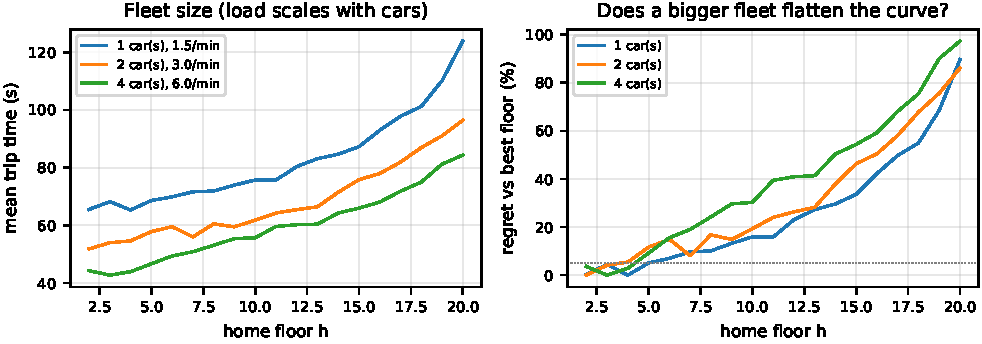
\includegraphics[width=\columnwidth]{figures/fleet.pdf}
\caption{One, two and four cars with a background load that scales with the
fleet (1.5 passengers/min per car). Left: mean trip time; right: regret
relative to the best floor. A bigger fleet lowers every floor and steepens the
curve in relative terms.}
\label{fig:fleet}
\end{figure}

\paragraph{Fleet.} Adding cars at constant load per car lowers the best
floor's time from \FleBestOne\,s (one car) to \FleBestTwo\,s (two) and
\FleBestFour\,s (four) --- and raises the middle floor's regret from
\FleRegMidOne\% to \FleRegMidTwo\% and \FleRegMidFour\%
(Figure~\ref{fig:fleet}). More cars remove waiting, and waiting was the part
of the trip that did not depend much on $h$; what remains is the ride, which
is distance. The intuition that a well-served building makes the floor
irrelevant is backwards: it makes the floor a larger share of what you feel.
